\documentclass{article}
\usepackage{122}

\usepackage{graphicx}
\usepackage{pgfplots}

\newcommand{\hr}{\par\vspace{.5\baselineskip}\noindent\hrulefill\par}

\title{Теория вероятности \\ Конспект семинара №4}

\begin{document}
  \maketitle

  \section*{№1}
  каждый из 2х стрелков имеет по 2 пули \\
  вероятность попадания $p$ \\
  поочерёдно выстрелы

  \begin{enumerate}[label=\realasbuk*)]
    \item победил 1ый стрелок (событие $A$)
    \item победил 2ый стрелок (событие $B$)
    \item победил никто (событие $C$)
    \item кончились патроны (событие $D$)
  \end{enumerate}

  \begin{enumerate}%[label=\realasbuk*)]
    \item $P(A) = P(A_1) + P(A_3) + P(A_5) = p + p \cdot \l(1-p\r)^2 + p \cdot \l(1-p\r)^4
      = p \cdot \l(1 + \l(1-p\r)^2 + \l(1-p\r)^4\r)$
    \item $P(B) = P(B_2) + P(B_4) + P(B_5) = \l(1-p\r) \cdot p + \l(1-p\r)^3 \cdot p + \l(1-p\r)^5 \cdot p
      = \l(1-p\r) \cdot p \cdot \l(1 + \l(1-p\r)^2 + \l(1-p\r)^4\r) $
    \item $P(C) = \l(1-p\r)^6$
    \item $P(D) = P(C) + p \cdot \l(1-p\r)^5 = \l(1-p\r)^5$
  \end{enumerate}

  \section*{№2}
  $G_1 : A-B-A$ \\
  $G_2 : B-A-B$ \\
  $A_i$ -- вероятность $A$ выиграть итый матч \\
  $B_i$ -- вероятность $B$ выиграть итый матч \\
  НИЧЕГО НЕПОНЯТНО

  \hr
  \section*{Схема Бернулли}
  $$ P_n(k) = С_n^k \cdot p^k \cdot \l(1-p\r)^{n-k} $$
  \begin{center}
    $P_n(k) $ -- это вероятность $k$ успехов в $n$ попытках
  \end{center}

  \section*{№3}
  <<успех это у нас промах... ну вот так вот>> \\
  $p = 0.2$ \qquad $n=5$ \\
  найти $P_n(k)$ где $0 \leq k \leq 5$

  \begin{enumerate}
    \item $P_5(0) = C^0_5 \cdot 0.2^0 \cdot 0.8^5 = 0.32769$
    \item $P_5(1) = C^1_5 \cdot 0.2^1 \cdot 0.8^4 = 0.4096$
    \item $P_5(2) = C^2_5 \cdot 0.2^2 \cdot 0.8^3 = 0.2048$
    \item $P_5(3) = C^3_5 \cdot 0.2^3 \cdot 0.8^2 = 0.0512$
    \item $P_5(4) = C^4_5 \cdot 0.2^4 \cdot 0.8^1 = 0.0064$
    \item $P_5(5) = C^5_5 \cdot 0.2^5 \cdot 0.8^0 = 0.00032$
  \end{enumerate}

  \begin{center}
    \begin{tikzpicture}
      \begin{axis}
        \addplot coordinates {(0, 0.32769)(1, 0.4096)(2, 0.2048)(3, 0.0512)(4, 0.0064)(5, 0.00032)};
      \end{axis}
    \end{tikzpicture}
  \end{center}


  \hr
  \section*{Условия}
  \includegraphics[page=45, width=0.3\textwidth]{./books/учебник теорвер.pdf} \hfill
  \includegraphics[page=46, width=0.3\textwidth]{./books/учебник теорвер.pdf} \hfill
  \includegraphics[page=47, width=0.3\textwidth]{./books/учебник теорвер.pdf} \hfill

  \section*{Ответы}
  \includegraphics[page=214, width=\textwidth, trim={0 5cm 0 7cm}, clip]{./books/учебник теорвер.pdf}

\end{document}
